% Created by tikzDevice version 0.12.4 on 2023-11-13 17:29:13
% !TEX encoding = UTF-8 Unicode
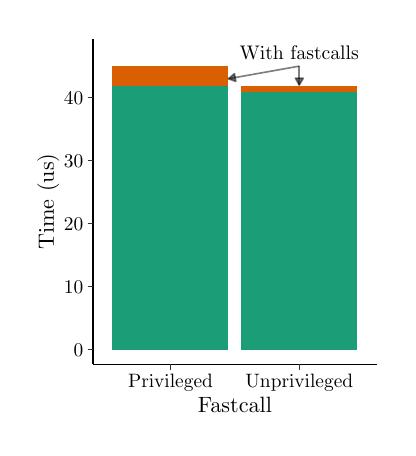
\begin{tikzpicture}[x=1pt,y=1pt]
\definecolor{fillColor}{RGB}{255,255,255}
\path[use as bounding box,fill=fillColor,fill opacity=0.00] (0,0) rectangle (130.09,144.54);
\begin{scope}
\path[clip] (  0.00,  0.00) rectangle (130.09,144.54);
\definecolor{drawColor}{RGB}{255,255,255}
\definecolor{fillColor}{RGB}{255,255,255}

\path[draw=drawColor,line width= 0.4pt,line join=round,line cap=round,fill=fillColor] (  0.00,  0.00) rectangle (130.09,144.54);
\end{scope}
\begin{scope}
\path[clip] ( 23.66, 22.85) rectangle (126.09,140.54);
\definecolor{fillColor}{RGB}{255,255,255}

\path[fill=fillColor] ( 23.66, 22.85) rectangle (126.09,140.54);
\definecolor{fillColor}{RGB}{217,95,2}

\path[fill=fillColor] ( 30.65,123.51) rectangle ( 72.55,130.58);
\definecolor{fillColor}{RGB}{27,158,119}

\path[fill=fillColor] ( 30.65, 28.20) rectangle ( 72.55,123.51);
\definecolor{fillColor}{RGB}{217,95,2}

\path[fill=fillColor] ( 77.20,121.13) rectangle (119.10,123.59);
\definecolor{fillColor}{RGB}{27,158,119}

\path[fill=fillColor] ( 77.20, 28.20) rectangle (119.10,121.13);
\definecolor{drawColor}{RGB}{0,0,0}

\path[draw=drawColor,draw opacity=0.50,line width= 0.6pt,line join=round] ( 72.55,126.08) -- ( 98.15,130.64);
\definecolor{fillColor}{RGB}{0,0,0}

\path[draw=drawColor,draw opacity=0.50,line width= 0.6pt,line join=round,fill=fillColor,fill opacity=0.50] ( 74.72,127.92) --
	( 72.55,126.08) --
	( 75.22,125.12) --
	cycle;

\path[draw=drawColor,draw opacity=0.50,line width= 0.6pt,line join=round] ( 98.15,123.81) -- ( 98.15,130.64);

\path[draw=drawColor,draw opacity=0.50,line width= 0.6pt,line join=round,fill=fillColor,fill opacity=0.50] ( 96.73,126.27) --
	( 98.15,123.81) --
	( 99.58,126.27) --
	cycle;
\definecolor{drawColor}{RGB}{0,0,0}

\node[text=drawColor,anchor=base,inner sep=0pt, outer sep=0pt, scale=  0.71] at ( 98.15,133.09) {With fastcalls};
\end{scope}
\begin{scope}
\path[clip] (  0.00,  0.00) rectangle (130.09,144.54);
\definecolor{drawColor}{RGB}{0,0,0}

\path[draw=drawColor,line width= 0.6pt,line join=round] ( 23.66, 22.85) --
	( 23.66,140.54);
\end{scope}
\begin{scope}
\path[clip] (  0.00,  0.00) rectangle (130.09,144.54);
\definecolor{drawColor}{RGB}{0,0,0}

\node[text=drawColor,anchor=base east,inner sep=0pt, outer sep=0pt, scale=  0.70] at ( 20.06, 25.79) {0};

\node[text=drawColor,anchor=base east,inner sep=0pt, outer sep=0pt, scale=  0.70] at ( 20.06, 48.55) {10};

\node[text=drawColor,anchor=base east,inner sep=0pt, outer sep=0pt, scale=  0.70] at ( 20.06, 71.32) {20};

\node[text=drawColor,anchor=base east,inner sep=0pt, outer sep=0pt, scale=  0.70] at ( 20.06, 94.08) {30};

\node[text=drawColor,anchor=base east,inner sep=0pt, outer sep=0pt, scale=  0.70] at ( 20.06,116.84) {40};
\end{scope}
\begin{scope}
\path[clip] (  0.00,  0.00) rectangle (130.09,144.54);
\definecolor{drawColor}{gray}{0.20}

\path[draw=drawColor,line width= 0.4pt,line join=round] ( 21.66, 28.20) --
	( 23.66, 28.20);

\path[draw=drawColor,line width= 0.4pt,line join=round] ( 21.66, 50.96) --
	( 23.66, 50.96);

\path[draw=drawColor,line width= 0.4pt,line join=round] ( 21.66, 73.73) --
	( 23.66, 73.73);

\path[draw=drawColor,line width= 0.4pt,line join=round] ( 21.66, 96.49) --
	( 23.66, 96.49);

\path[draw=drawColor,line width= 0.4pt,line join=round] ( 21.66,119.26) --
	( 23.66,119.26);
\end{scope}
\begin{scope}
\path[clip] (  0.00,  0.00) rectangle (130.09,144.54);
\definecolor{drawColor}{RGB}{0,0,0}

\path[draw=drawColor,line width= 0.6pt,line join=round] ( 23.66, 22.85) --
	(126.09, 22.85);
\end{scope}
\begin{scope}
\path[clip] (  0.00,  0.00) rectangle (130.09,144.54);
\definecolor{drawColor}{gray}{0.20}

\path[draw=drawColor,line width= 0.4pt,line join=round] ( 51.60, 20.85) --
	( 51.60, 22.85);

\path[draw=drawColor,line width= 0.4pt,line join=round] ( 98.15, 20.85) --
	( 98.15, 22.85);
\end{scope}
\begin{scope}
\path[clip] (  0.00,  0.00) rectangle (130.09,144.54);
\definecolor{drawColor}{RGB}{0,0,0}

\node[text=drawColor,anchor=base,inner sep=0pt, outer sep=0pt, scale=  0.70] at ( 51.60, 14.43) {Privileged};

\node[text=drawColor,anchor=base,inner sep=0pt, outer sep=0pt, scale=  0.70] at ( 98.15, 14.43) {Unprivileged};
\end{scope}
\begin{scope}
\path[clip] (  0.00,  0.00) rectangle (130.09,144.54);
\definecolor{drawColor}{RGB}{0,0,0}

\node[text=drawColor,anchor=base,inner sep=0pt, outer sep=0pt, scale=  0.80] at ( 74.87,  5.56) {Fastcall};
\end{scope}
\begin{scope}
\path[clip] (  0.00,  0.00) rectangle (130.09,144.54);
\definecolor{drawColor}{RGB}{0,0,0}

\node[text=drawColor,rotate= 90.00,anchor=base,inner sep=0pt, outer sep=0pt, scale=  0.80] at (  9.51, 81.69) {Time (us)};
\end{scope}
\end{tikzpicture}
